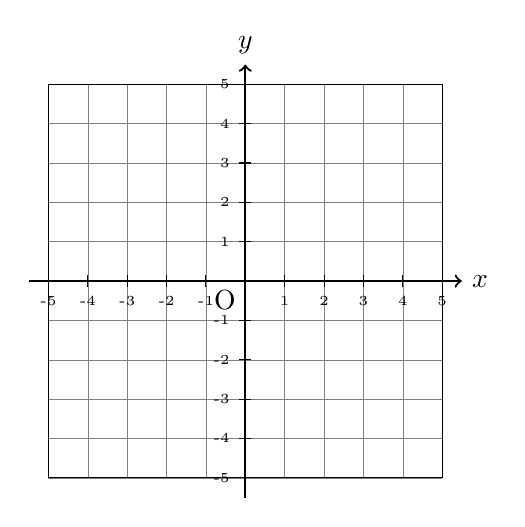
\begin{tikzpicture}[scale=0.5]
  \draw[step=1.0,gray,very thin] (-5,-5) grid (5,5);
  \draw[step=5.0,black,thin] (-5,-5) grid (5,5);
  \draw[thick,->] (-5.5,0) -- (5.5,0) node[right] {$x$};
  \draw[thick,->] (0,-5.5) -- (0,5.5) node[above] {$y$};
  \node[below left] at (0,0) {O};
  \foreach \x in {-5,-4,-3,-2,-1,1,2,3,4,5} {
    \draw (\x,0.15) -- (\x,-0.15) node[below] {\tiny\x};
  }
  \foreach \y in {-5,-4,-3,-2,-1,1,2,3,4,5} {
    \draw (0.15,\y) -- (-0.15,\y) node[left] {\tiny\y};
  }
\end{tikzpicture}